\newpage
\section{Badania operatorów}

\subsection{Wybrane ćwiczenia}
Dla każdego z wybranych do automatycznej oceny zadań w tabeli \ref{tab:ocena-funkcje}, w trakcie szkolenia wykonuje się ćwiczenie które ma na celu opanowanie tej umiejętności. Zgodnie z wymogami przytoczonymi w rozdziale \ref{sec:tradycyjny-egzamin}, zawis wykonywany jest w określonym miejscu w kilku orientacjach BSP względem operatora. W doświadczeniach autora instruktor określa miejsce zawisu poprzez znak na ziemi lub umieszczenie niewielkiego obiektu, przykładowo pachołka drogowego. Ćwiczenie rozpoczyna się od zawisu tyłem do operatora --- czyli przód BSP pokrywa się z kierunkiem patrzenia. Wtedy sterowanie jest najłatwiejsze, ponieważ pochylenie i przechylenie BSP odbywa się w tę samą stronę jak wychylenie drążka sterowania. Po wybranym przez siebie czasie, instruktor określa kolejny kierunek w którym należy zwrócić przód BSP. Oprócz tego ćwiczy się zachowanie stałej wysokości, jednak często nie jest określone jaka musi być dokładnie. Z tego powodu w tamach tego ćwiczenia, jako wzorcową wartość wysokości przyjmowana jest ta którą miał BSP kiedy po raz pierwszy znalazł się w poziomej odległości 0,5~m od wyznaczonego miejsca.

Kolejnym wykonywanym ćwiczeniem może być przelot po obwodzie kwadratu, utrzymując przód w kierunku ruchu. Sprawdza umiejętność lotu po prostej w czterech różnych orientacjach BSP. Narożniki kwadratu mogą być oznaczone podobnie jak miejsce wykonywania zawisu. Podobnie jak inne szczegóły szkolenia i egzaminu, długość boku tego kwadratu powinna byc dostosowana do statku powietrznego. Na podstawie doświadczenia autora, dla wielowirnikowca średniej wielkości tj. masie startowej 3~kg zostanie wykorzystany kwadrat o boku 8~m. Umiejscowienie operatora nie jest szczególnie ważne, dopóki znajduje się w bezpiecznej odległości od oblatywanego obszaru. Oczekiwane jest że wykona ćwiczenie nie przemieszczając się za BSP. Poglądowy schemat ilustrujący to ćwiczenie zamieszczono na rysunku \ref{fig:kwadrat}.

\begin{figure}[!h]
    \centering 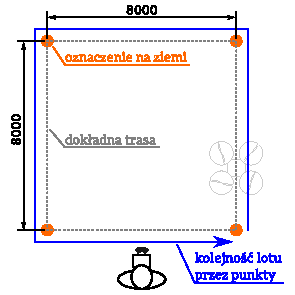
\includegraphics[width=0.6\linewidth]{kwadrat.pdf}
    \caption{Schemat ćwiczenia lotu wzdłuż prostych}
    \label{fig:kwadrat}
\end{figure}

Umiejętności wprowadzenia w zakręt, krążenia, oraz wyprowadzenia z zakrętu według doświadczeń autora są rozwijane w ramach wykonywania jednego ćwiczenia. W przeciwieństwie do manewrów opisywanych do tej pory, w tym przypadku wymagana jest pewna prędkość postępowa. Lot po okręgu wymaga wytworzenia przyspieszenia dośrodkowego o wartości proporcjonalnej do prędkości lotu. Wymagając pewnej minimalnej prędkości, utrzymanie przodu BSP w kierunku ruchu wymaga wtedy odpowiedniego przechylenie wielowirnikowca do środka zakrętu. Z tego powodu ćwiczenie rozpoczyna się od rozpędzenia w wybranym kierunku. Następnie wykonywany jest zakręt, lot wokół okręgu, wyjście z zakrętu i wyhamowanie do zawisu. Zwraca się głównie uwagę na zakreślenie równomiernego koła wokół obszaru wykonywania ćwiczeń, oraz zachowanie dynamicznego charakteru manewru. Dla stosowanego modelu wielowirnikowca arbitralnie dobrano promień koła 5~m, który po sprawdzeniu w symulacji przez autora został uznany za adekwatny. Wzajemne położenie trasy przelotu i naziemnych oznaczeń w widoku z góry ilustruje rysunek \ref{fig:kolo}.

\begin{figure}[!h]
    \centering 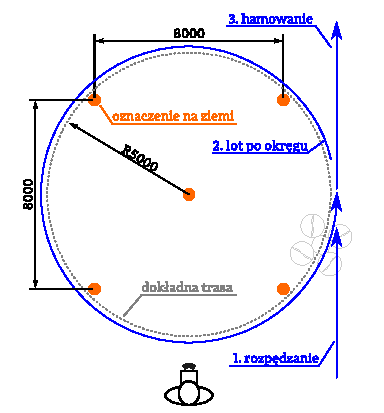
\includegraphics[width=0.8\linewidth]{kolo.pdf}
    \caption{Schemat ćwiczenia lotu w zakręcie po okręgu}
    \label{fig:kolo}
\end{figure}

\subsubsection{Implementacja w aplikacji}
Zgodnie z założeniami poczynionymi na etapie projektowania aplikacji wizualnej, dla każdego ćwiczenia przygotowano osobną scenę, w nomenklaturze silnika Unreal Engine nazywaną ,,mapą''. Aby oznaczyć miejsce zawisu umieszczono pachołek drogowy o wysokości 600~mm w odległości 7~m od operatora. Bezpośrednio nad nim znajduje się niewidoczny w trakcie ćwiczenia prostopadłościan, na rysunku \ref{fig:examhover} reprezentowany zielonymi liniami. Wlot BSP do tego obszaru rozpoczyna ocenę, zapisuje obecną wysokość jako referencyjną i rozpoczyna pomiar czasu. Niebieski znacznik orientacji umieszczony pomiędzy miejscem zawisu a operatorem wskazuje kierunek w którym należy skierować przód statku powietrznego. Po upływie 10 sekund od wejścia w zawis nad pachołkiem, ocena jest zatrzymywana, znacznik obracany o 90~°. Operator ma 5 sekund na odchylenie w nowym kierunku, po czym ocena jest wznawiana. Rozpoczęcie oceny każdorazowo jest sygnalizowane krótkim dźwiękiem. Taki cykl jest wykonywany cztery razy, dla kolejnych kursów różniących się o 90~°.

\begin{figure}[!h]
    \centering 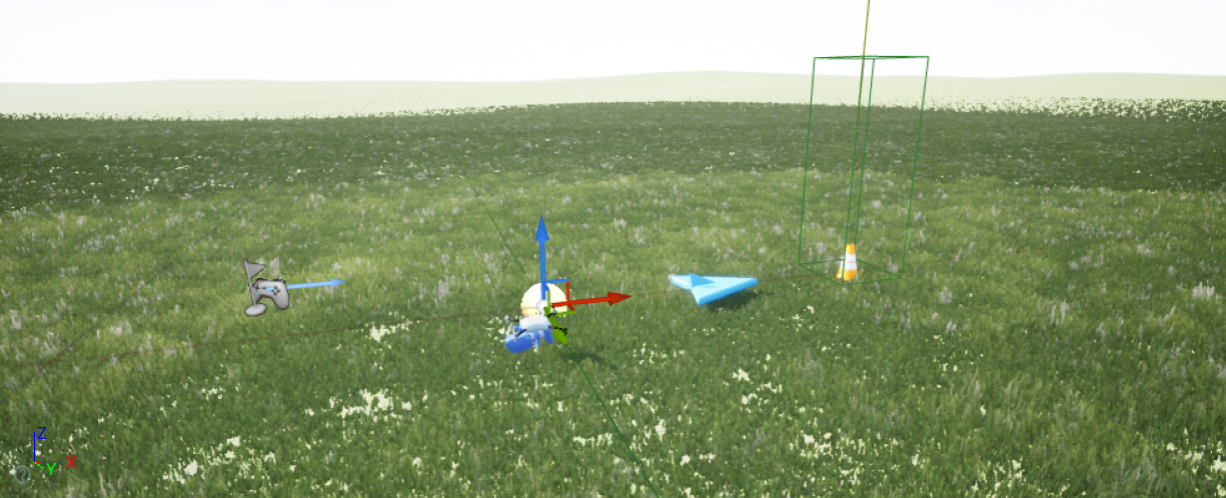
\includegraphics[width=\linewidth]{examhover.png}
    \caption{Zrzut ekranu obszaru do wykonywania zawisu}
    \label{fig:examhover}
\end{figure}

Kolejne wykonywane ćwiczenie ma na celu opanowanie lotu po prostej. Identyczne pachołki drogowe jak dla oznaczenia miejsca zawisu zostały rozmieszczone w sposób opisany na rysunku \ref{fig:kwadrat}. Na wysokości 2~m nad ziemią ułożono trasę składającą się z czterech odcinków łączących kolejne wierzchołki kwadratu. Ponieważ ćwiczenie rozpoczyna się i kończy w tym samym miejscu, na każdym narożniku dodano bramki kontrolne, na rysunku \ref{fig:examsquare} widoczne jako półprzezroczyste niebieskie koła o średnicy 2~m. Poprawne ukończenie zadania wymaga przelotu przez każdą z nich. Aby czytelniej przekazać przebieg trasy, na początku ćwiczenia widoczna jest tylko bramka startu. W momencie gdy BSP znajdzie się w pobliżu przeciwległego narożnika trasy, start jest ukrywany, a zamiast tego włączana jest czerwona bramka końca.

\begin{figure}[!h]
    \centering 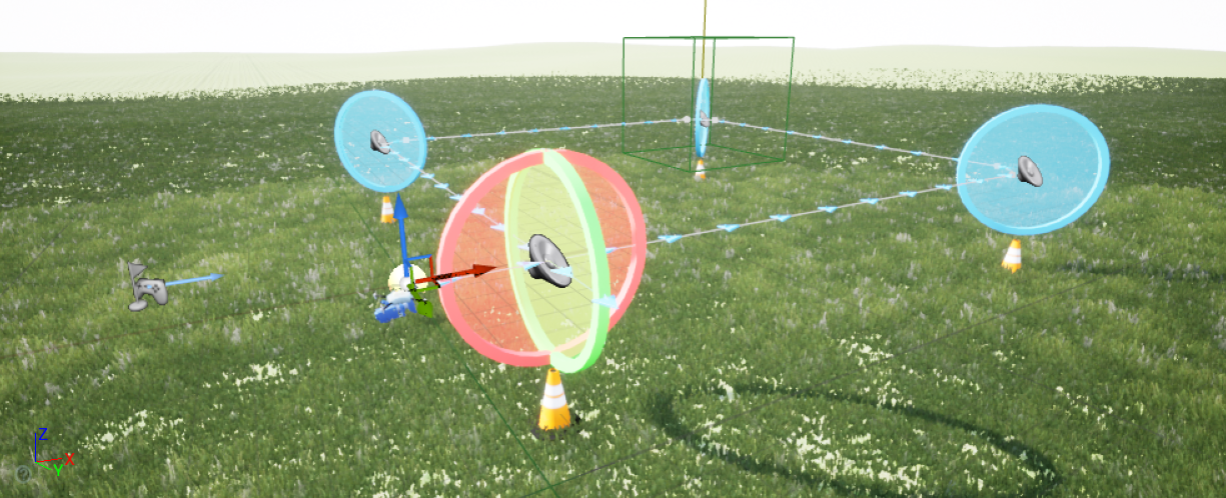
\includegraphics[width=\linewidth]{examsquare.png}
    \caption{Zrzut ekranu obszaru do lotu po obwodzie kwadratu}
    \label{fig:examsquare}
\end{figure}

Ćwiczenie lotu w zakręcie zostało zaimplementowane w sposób bardzo zbliżony do lotu wzdłuż obwodu kwadratu. Wytyczono okrąg o średnicy i położeniu zgodnym z rysunkiem \ref{fig:kolo}. Ponieważ ćwiczenie wykonywane jest z większą prędkością, a mniejszą precyzją, podczas szkolenia praktycznego często odbywa się nieco wyżej niż pozostałe. Aby to odwzorować, trasa znajduje się na wysokości 4~m nad terenem, a bramki mają średnicę 3~m. Wygląd mapy w edytorze przedstawia rysunek \ref{fig:examcircle}. Także w tym przypadku, podczas lotu początkowo widoczna jest tylko bramka oznaczająca początek próby, a po przeleceniu połowy trasy tylko bramka końcowa.

\begin{figure}[!h]
    \centering 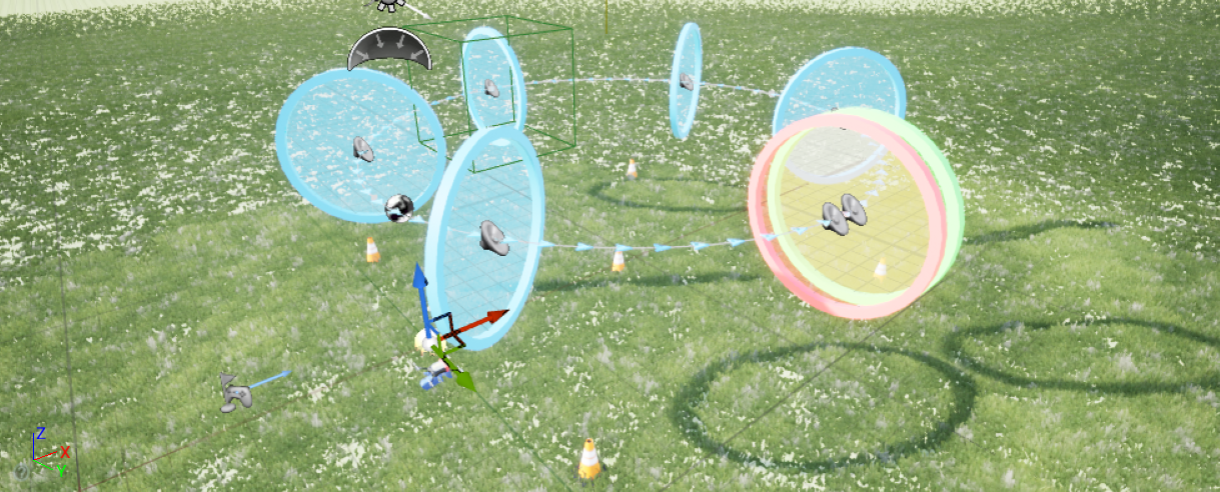
\includegraphics[width=\linewidth]{examcircle.png}
    \caption{Zrzut ekranu obszaru do lotu w zakręcie}
    \label{fig:examcircle}
\end{figure}

\subsection{Przebieg eksperymentu}
\begin{todo}
    Wybrane kilka osób, o różnym stopniu doświadczenia w pilotażu BSP. Ta sama liczba podejść do każdego z zadań.
\end{todo}

We wszystkich próbach wykorzystywany był domyślny model dynamiczny wielowirnikowca zaimplementowany w bibliotece ArduPilot SITL\cite{sitl-model}. Najważniejsze parametry modelu przedstawiono w tabeli \ref{tab:sitl-model}. Należy zrócić uwagę, że ponieważ modelowana jest jedna konfiguracja elektrycznego statku powietrznego, masa pozostaje stała --- nie ma potrzeby rozdzielać jej na maksymalną, suchą etc. Operatorzy sterowali modelem wykorzystując rzeczywisty nadajnik zdalnego sterowania \emph{FrSKY Horus X10 Express} widoczny na rysunku \ref{fig:frsky-horus}. Drążki sterowe były ustawione w układzie \emph{Mode 2}, który jest najbardziej popularny\cite{mcnabb2021}. Lewy drążek wychylany w lewo lub prawo powodował odpowiadające sterowanie w osi odchylenia. Wychylenie lewego drążka do góry zwiększa wysokość, a w dół obniża lot. Prawy drążek sterowy ma przypisane osie pochylenia i przechylenia identycznie jak w samolotach. Trzy osie, z wyjątkiem sterowania wysokością są wyposażone w sprężyny które przywracają je do położenia centralnego.
\begin{table}[!h] \centering
    \caption{Charakterystyczne wielkości modelowanego BSP}
    \label{tab:sitl-model}

    \begin{tabular}{|l | r|l |}
    \hline
    Cecha charakterystyczna & Wielkość & Jednostka \\ \hline \hline
    Masa & 3 & kg \\ \hline
    Moment bezwł. $ X $ & 0,0230 & $ \text{kg}\cdot\text{m}^2 $ \\ \hline
    Moment bezwł. $ Y $ & 0,0230 & $ \text{kg}\cdot\text{m}^2 $ \\ \hline
    Moment bezwł. $ Z $ & 0,0459 & $ \text{kg}\cdot\text{m}^2 $ \\ \hline
    Konfiguracja & \multicolumn{2}{c|}{\emph{quadrotor X}} \\ \hline
    Długość & 600 & mm \\ \hline
    Szerokość & 600 & mm \\ \hline
    Średnica śmigła & 350 & mm \\ \hline
    Liczba śmigieł & 4 & szt. \\ \hline
    Rozstaw śmigieł & 250 & mm \\ \hline
    Moc pobierana w zawisie & 354 & W \\ \hline
  \end{tabular}
\end{table}

\begin{figure}[!h]
    \centering 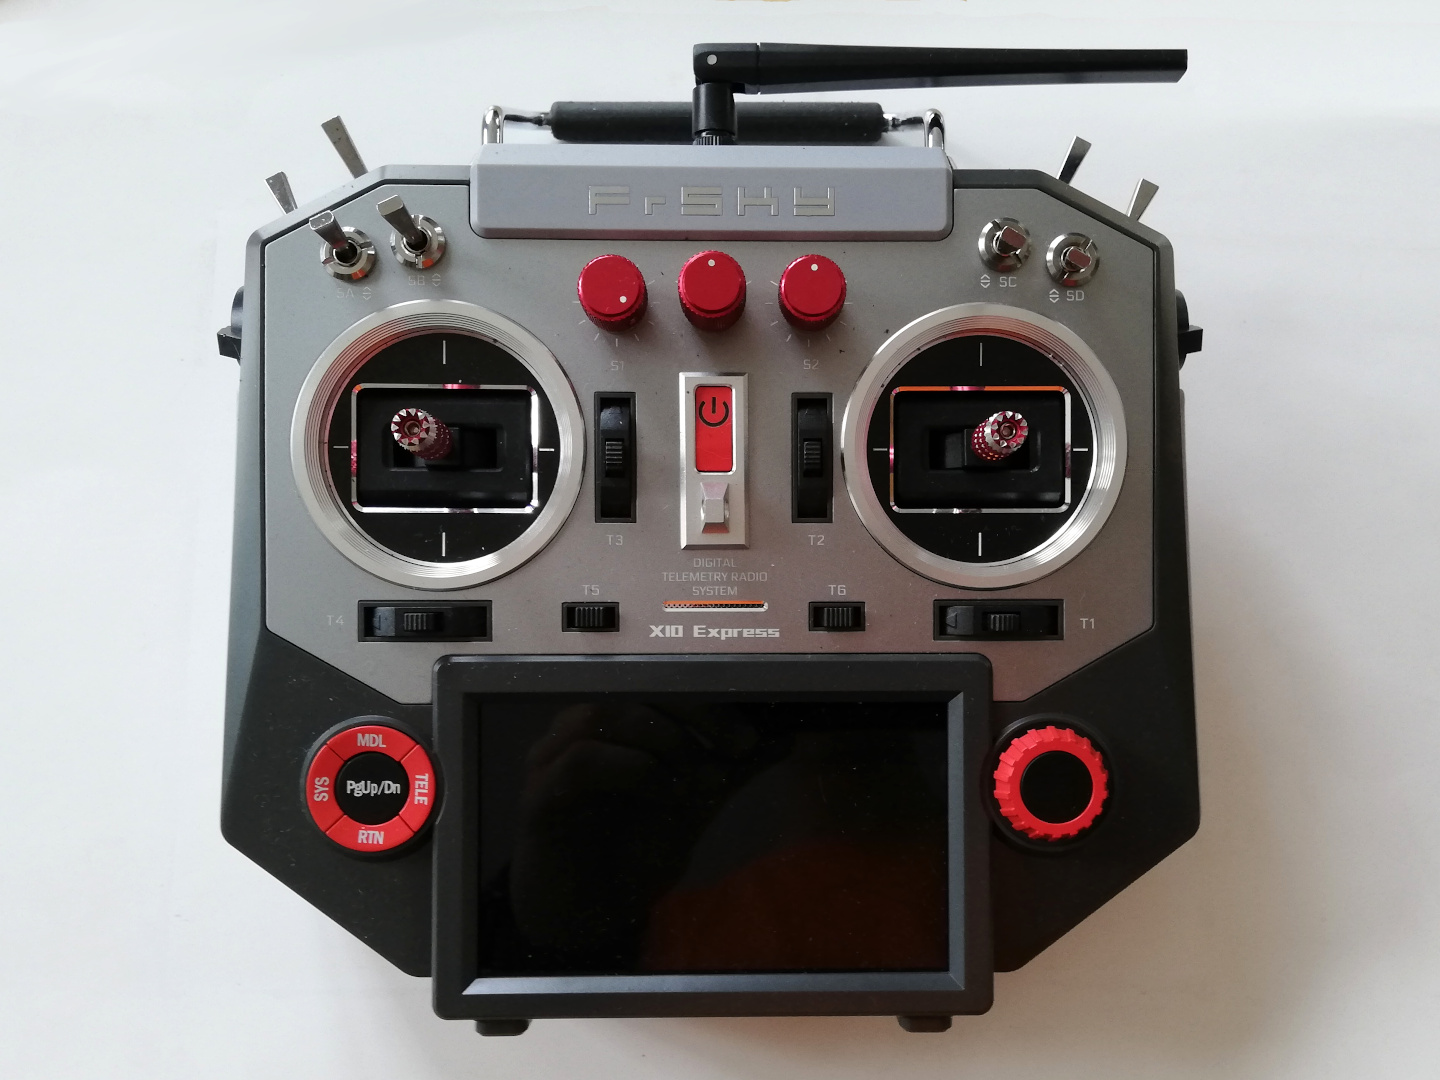
\includegraphics[width=0.8\linewidth]{frsky-horus.jpg}
    \caption{Wykorzystywany nadajnik zdalnego sterowania}
    \label{fig:frsky-horus}
\end{figure}

\subsection{Wyniki}
\begin{todo}
    Zestawienie wyników poszczególnych operatorów, w kolejnych podejściach do danego zadania. Wykres \emph{learning curve}.
\end{todo}